
\section{Results}
\label{sec:results}


\begin{wrapfigure}{r}{0.475\linewidth}
\vspace{-14pt}
\centering
\includegraphics[width=0.8\linewidth]{Chapter02/fig/legend.pdf}
% \vspace{-15pt}
\caption{The 2D tessellation of 8D ternary vector space used in Fig.~\ref{fig:sim}.}
\label{fig:tesselation}
\vspace{-1em}
\end{wrapfigure}


To test the effects of morphology on fitness and sim2real transfer success, it is useful to first visualize the design space. 
However, because there are eight cartesian voxel coordinates in the chosen workspace, the design space here is eight dimensional, which is difficult to draw (let alone conceptualize) without dimensionality reduction.
By nesting the dimensions of a search space onto a single plot (Fig.~\ref{fig:tesselation}), the entire space can be visualized as a 2D heatmap.
This strategy was used by \citet{cully2015robots} to neatly visualize the predicted fitness of a very large library of control policies, as a function of the time a robot's six limbs were in contact with the simulated ground plane: 6D quinary control space was mapped to 2D, by nesting pairs of dimensions within each other.



\begin{figure}[t]
    % \vspace{-2em}
    \centering
    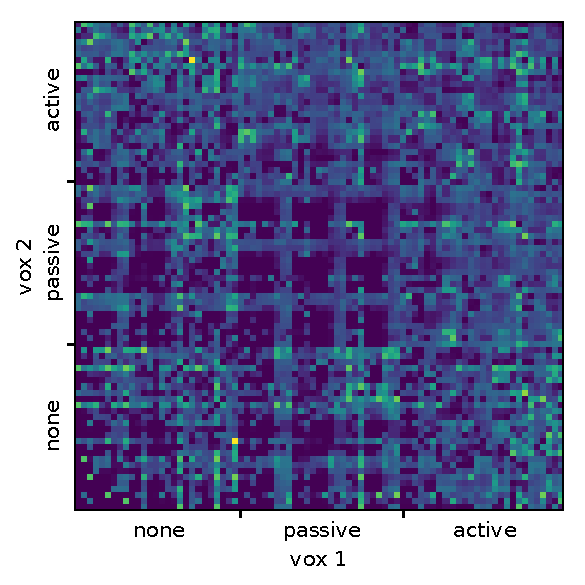
\includegraphics[width=0.7\linewidth]{Chapter02/fig/design_space.pdf}
    % \vspace{-2em}
    \caption{\textbf{Simulating modular soft robots.}
    The design space is plotted as a heatmap, containing one cell for each of the 6561 possible configurations.
    Lighter colored cells are fitter designs (Eq.~\ref{eq:fitness}).
    Each design is defined by a vector of eight ternary values, indicating what kind of voxel (none, passive, or active) the design contains at the eight lattice points in the $2\times2\times2$ workspace.
    The 8D ternary vector is reduced to a 2D heatmap by nesting pairs of dimensions within each other: four, nested $3\times3$ grids result in a $3^4\times3^4=81\times81$ overall heatmap.
    }
    \label{fig:sim}
    % \vspace{-1em}
\end{figure}



Here, the 8D ternary morphology space was reduced to 2D by plotting pairs of dimensions nested within each other (Fig.~\ref{fig:sim}).
The pixel in the exact center of Fig.~\ref{fig:sim}, for instance, represents the configuration consisting entirely of passive voxels, and thus cannot locomote ($F=0$).
Likewise, the pixel in the top right-hand corner of the heatmap represents the configuration of all active voxels (Fig.~\ref{fig:transfer}d), which actuated symmetrically in phase, and thus (given its flat ventral surface) could not locomote across the flat ground plane ($F=0$).
Finally, the pixel in the bottom left-hand corner contains no voxels at all, and thus $F=0$.


For locomotion, a good design obviously needs to have a body, rather than none at all.
With open-loop, in-phase actuation, designs also need to have asymmetrical mass and/or actuator distributions, or they will not generate any forward movement.
However it is not clear, even for this minimal design space, exactly which asymmetrical designs will yield the highest fitness.
Yet we can see small clusters and lines of similarly colored pixels in Fig.~\ref{fig:sim}, representing morphologically similar designs with similar fitness.
This suggests that these configurations and substructures would be relatively stable under random mutations or errors in fabrication.


Because fitness was measured by displacement in any direction away from the origin (Eq.~\ref{eq:fitness}), there are four configurations---rotations, in the x,y plane, of a single geometry and distribution of passive and active voxels---with different behaviors (they moved in different directions) but very similar (if not identical) fitness.
There were also some configurations that, when rotated upward (in the x,z or y,z plane) fell into the same basic orientation and behavior but with a slightly different heading.
Thus, configurations with similar fitness (similarly colored pixels) are reflected across multiple, nested planes of symmetry in Fig.~\ref{fig:sim}.
These symmetries can also be seen in the manufactured robots (Fig.~\ref{fig:teaser}b).
The uniqueness of designs (i.e., the size of the search space of morphologies) is therefore a function of how behavior is measured.



\begin{figure*}[t]
    \centering
    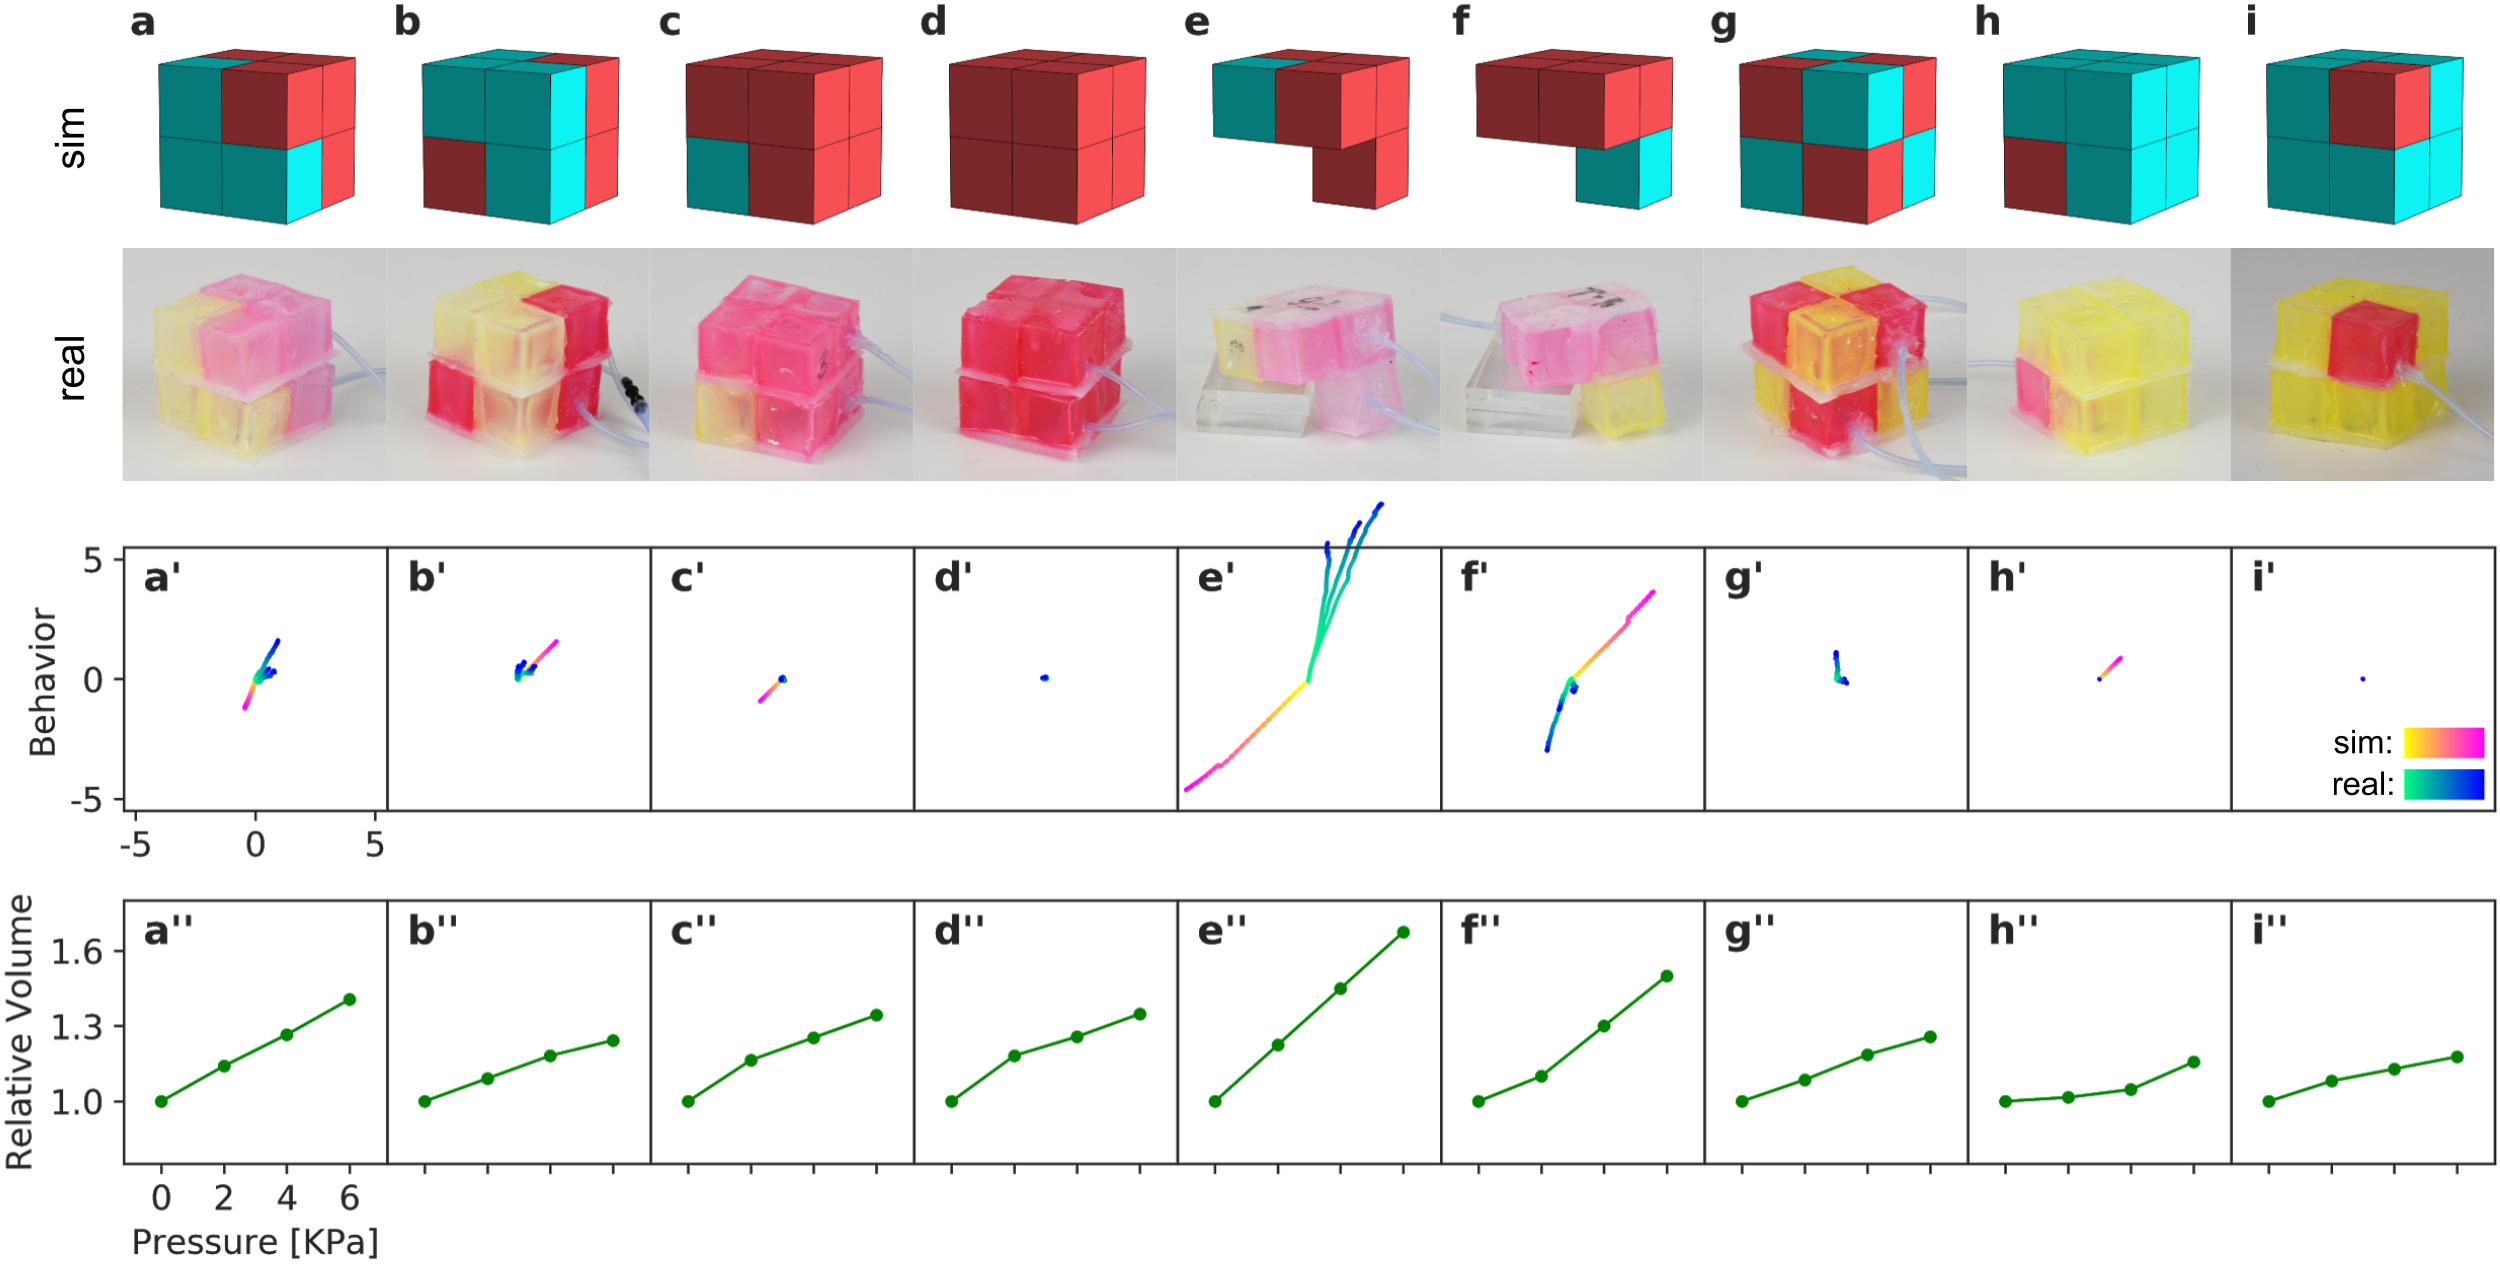
\includegraphics[width=\linewidth]{Chapter02/fig/YaleTraces2.png}
    % \vspace{-1.75em}
    \caption{\textbf{Measuring transferal from simulation to reality}.
    Nine designs (\textbf{a-i}) were evaluated three times each in reality (green-to-blue gradient colored curves in \textbf{a\textquotesingle-i\textquotesingle}).
    The behavioral trajectories start at the origin (green) and end at the robot's final XY destination (blue) (in centimeters).
    The simulated movement tracks (yellow-to-pink curves) are superimposed on top of the real ones.
    The relative volume (normalized by rest volume) was also recorded for each design at four points during actuation under water (\textbf{a\textquotesingle\textquotesingle-i\textquotesingle\textquotesingle}).
    % The two designs that displaced farthest in the plane (e and f) also achieved the largest volumetric expansion.
    The simulated and real behavior of designs e and f can be observed here:
    \href{https://youtu.be/UqjvmkYa9u4}{\color{blue}\tt\textbf{youtu.be/UqjvmkYa9u4}}.
    }
    \label{fig:transfer}
    % \vspace{-1.25em}
\end{figure*}
 

\begin{figure}[t]
    \centering
    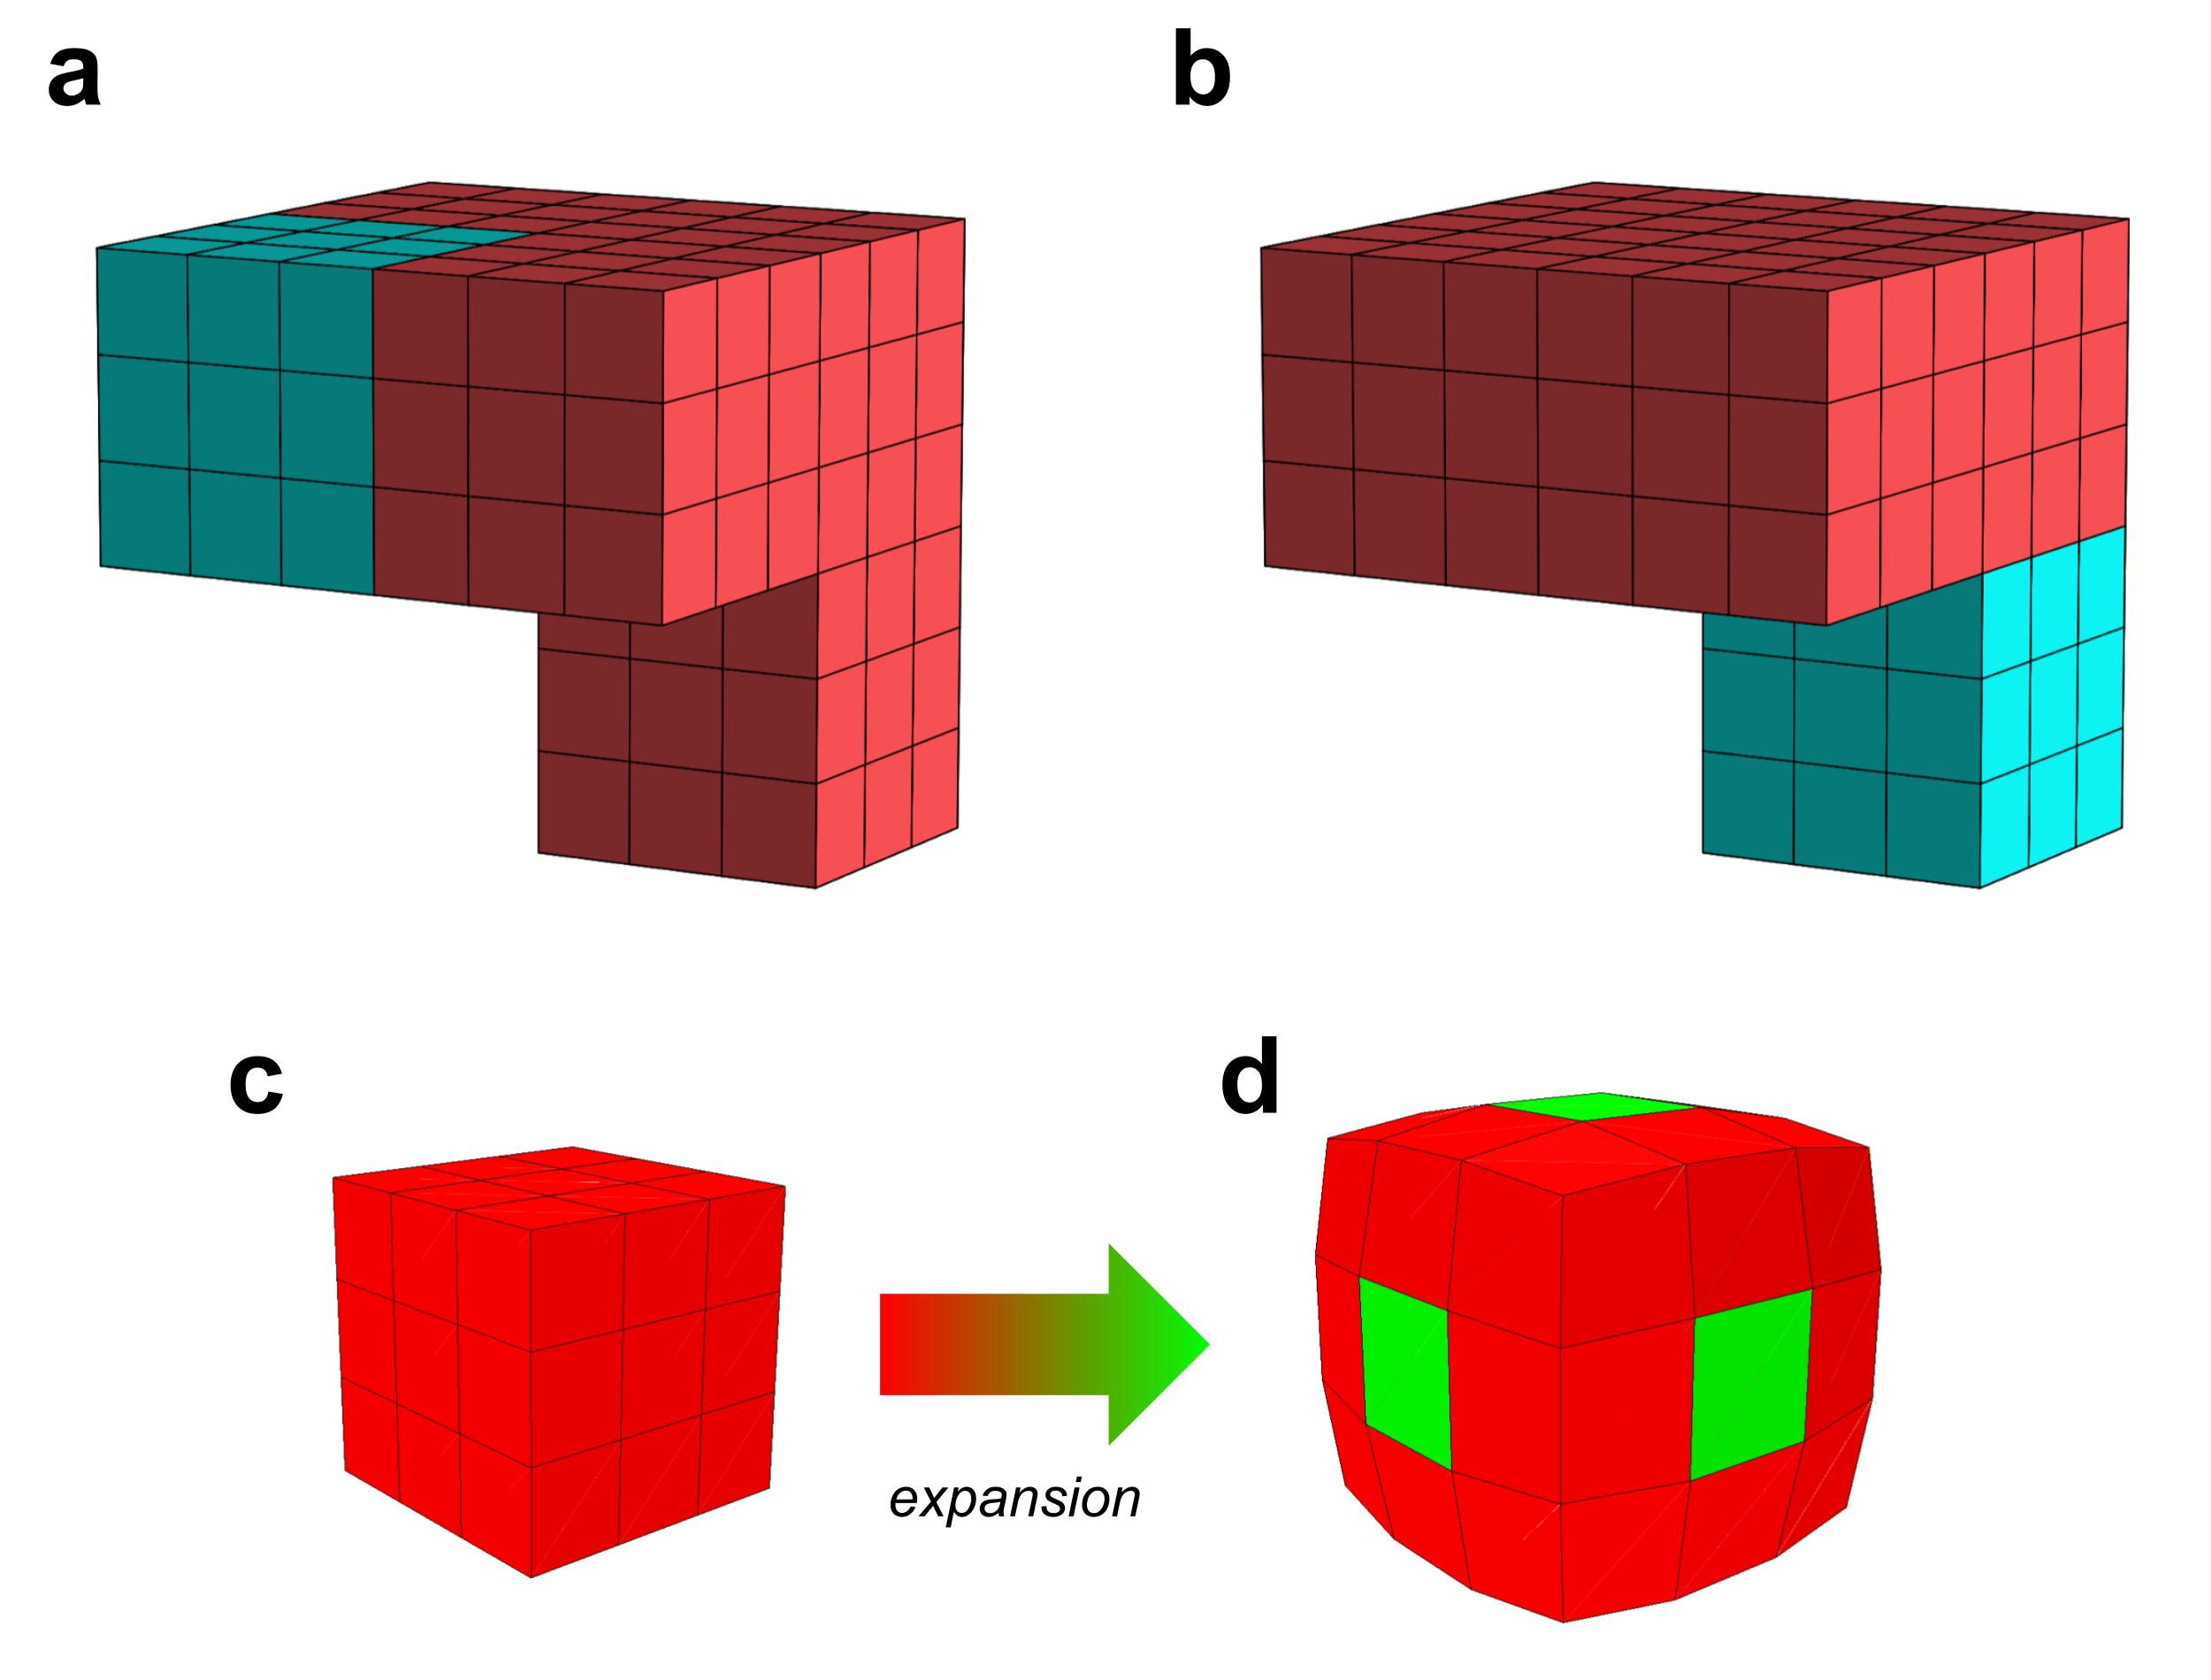
\includegraphics[width=0.65\linewidth]{Chapter02/fig/Yale_High_Res_Sim.jpg}
    % \vspace{-1em}
    \caption{A higher resolution model in which each silicone voxel is approximated by a 3-by-3-by-3 group of simulated subvoxels: a high-res voxel.
    The design in \textbf{a} and \textbf{b} are high-res instantiations of those in Figs.~\ref{fig:transfer}e and \ref{fig:transfer}f, respectively. 
    Spherical volumetric expansion in a high-res voxel (\textbf{c}) was approximated by increasing the rest length between the centermost subvoxel and the subvoxels at center of each face (green subvoxels in \textbf{d}).
    }
    \label{fig:hi_res_sim}
    % \vspace{-1.25em}
\end{figure}



Fig.~\ref{fig:transfer} shows the behavior of nine different designs in simulation and reality.
The real robot was actuated 90 times at 6 kPa pressure on a surface covered with cornstarch 
(Argo\textregistered, ACH Food Companies, Inc.) 
to reduce friction, and is compared to 23 simulated actuation cycles.
Seven of the nine designs filled the cubic workspace with passive and active voxels, while the other two share a more complex geometry: a single-voxel limb attached to the face of a 2-by-2 plane of voxels (Fig.~\ref{fig:transfer}e,f).
In one, the limb is active (Fig.~\ref{fig:transfer}e), in the other it is passive (Fig.~\ref{fig:transfer}f).
These two designs achieved the two highest fitness scores (Eq.~\ref{eq:fitness}), in both simulation and reality.

By this measure, the reality gap appears small.
However, these simulated designs move very differently from their manufactured equivalents.
The simulated morphology in Fig.~\ref{fig:transfer}e pushes off its active limb, whereas in reality the design uses its limb to pull itself forward, in the opposite direction.
Likewise, the simulated morphology in Fig.~\ref{fig:transfer}f pushes off its active 2-by-2 torso, whereas in reality the design uses its torso to pull itself forward, in the opposite direction.

\citet{majidi2013influence} showed that the interfacial shear strength and coefficient of friction of the surface on which their soft robot undulated determined the direction of locomotion. They decomposed friction into load- and area controlled terms for point and surface contacts, respectively. 
On slippery surfaces with low interfacial shear resistance, the robot anchored about the point contact (expanded section) for locomotion and pulled its surface contact (passive segment). However, on surfaces with high interfacial shear resistance, the robot anchored about the surface contact and pulled the point contact toward it. 
We hypothesize that such differences in tribological properties could have caused our designs to move in opposite directions in simulation and reality.

In an attempt to test this hypothesis and reduce the simulation-reality discrepancies that cause the virtual configurations in Fig.~\ref{fig:transfer} to move differently than their physical realizations, we performed a grid search of various simulation hyperparameters, including the coefficients of static and kinetic friction.
However, we could not identify a pair of friction coefficients that resulted in correct movement heading for all nine of the behaving designs (Fig.~\ref{fig:transfer}a\textquotesingle-i\textquotesingle).
This could be due to either low precision or low accuracy of the model.
To isolate and test the former possibility, we increased the resolution of the simulated surface contact geometry by modeling each silicone voxel as a 3-by-3-by-3 group of simulated ``subvoxels'' (Fig.~\ref{fig:hi_res_sim}),
and then re-ran the parameter sweep.
Still, we could not find friction settings in which the simulated movement direction matched the ground truth across all designs simultaneously.
This suggests that the accuracy of Coulomb friction model may be insufficient to model this type of movement.

The Coulomb approximation assumes that friction is simply proportional to the vertical component $N$ of the reaction force, and independent of the contact area. 
However, friction is also a function of the surface area and interfacial shear strength $\tau$, a fixed constant which is mostly governed by adhesion or mechanical interlocking between the contacting surfaces. 
A better model would thus consider friction as a function of both the normal force and the interfacial shear strength.
However, before fundamentally changing the simulator,
we plan to evaluate designs in noisy environments with imperfect control over actuation characteristics to avoid ascribing high fitness to designs that exploited unrealistic properties of the simulation \cite{jakobi1995noise}.
Additionally, data from reality could be used to automatically tune  the geometry and resolution of the simulated finite elements \cite{bongard2006resilient}, or to predict the kinds of behaviors that are more likely to successfully transfer \cite{koos2012transferability}, and which should be tested next \cite{bongard2006resilient}. 
Concurrently, we are investigating additional physical surfaces with varied tribological properties in an attempt to match reality to simulation.



% The best design achieved the largest volumetric expansion (Fig.~\ref{fig:transfer}a\textquotesingle\textquotesingle)...




